\chapter{直升机协同吊挂试验试飞}
\section{引言}
\begin{figure}[htb!]
    \centering
    
% \documentclass{article}
% \usepackage{xeCJK}
% \usepackage{tikz}
% \usetikzlibrary{shapes.geometric,arrows}
% \usetikzlibrary{fit}
% \usetikzlibrary{backgrounds}

% \tikzstyle{arrow}     = [thick,->,>=stealth]
% \tikzstyle{arrow_double}  = [thick,<->,>=stealth]
% \tikzstyle{startstop} = [rectangle, rounded corners, minimum width=2.5cm, minimum height=1cm, text centered, draw=black, fill=green!30]
% \tikzstyle{process} = [rectangle, rounded corners, text centered, draw = black, minimum width = 2.5cm, minimum height = 1cm]
% \tikzstyle{process_red} = [rectangle, rounded corners, text centered, draw = black, minimum width = 2.5cm, minimum height = 1cm, fill = red!30]
% \tikzstyle{process_orange} = [rectangle, rounded corners, text centered, draw = black, minimum width = 2.5cm, minimum height = 1cm, fill = orange!30]
% \tikzstyle{process_blue} = [rectangle, rounded corners, text centered, draw = black, minimum width = 2.5cm, minimum height = 1cm, fill = blue!30]
% \tikzstyle{process_green} = [rectangle, rounded corners, text centered, draw = black, minimum width = 2.5cm, minimum height = 1cm, fill = green!30]
% \tikzstyle{process_purple} = [rectangle, rounded corners, text centered, draw = black, minimum width = 2.5cm, minimum height = 1cm, fill = purple!20]
% \tikzstyle{decision}  = [diamond,shape aspect=2.5, minimum width=3cm, minimum height=1cm, inner xsep=0,text centered, draw=black, fill=red!30]

% \begin{document}


    \begin{tikzpicture}[node distance = 2cm]

        \node [startstop] (start) {开始};

        \node [process_blue, below of = start] (control) {理论实现};

        \node [process_orange,  xshift = 7cm, yshift = 0cm] (control_total) {基于Mavros的方法实现};
        \node [process_orange, below of = control_total](reality){控制律实现};
        \node [process_orange, below of = control_total, xshift = -3cm](env){环境搭建};
        \node [process_orange, below of = control_total, xshift = 3cm](ros){数据通信};
        \node [process_orange, below of = reality](safe) {飞行安全与可实现性};
        \begin{scope}[on background layer,label distance=1cm] 
            \node (back_control) [draw=black!50,dashed,thick,fill=black!10,fit=(control_total) (reality) (env) (ros) (safe) ] {};
        \end{scope}
        \draw [arrow] (control_total.south) --++ (0,-0.5) -| (env);
        \draw [arrow] (control_total.south) --++ (0,-0.5) -| (reality);
        \draw [arrow] (control_total.south) --++ (0,-0.5) -| (ros);
        \draw [arrow] (env.south) --++ (0,-0.5) -| (safe.north);
        \draw [arrow] (reality.south) --++ (0,-0.5) -| (safe.north);
        \draw [arrow] (ros.south) --++ (0,-0.5) -| (safe.north);
        \draw [arrow_double] (control) -- (back_control);

        \node [process_blue,below of = control, yshift = -3cm] (gazebo) {仿真验证};
        \node [process_green, right of = gazebo, xshift = 2cm, yshift = 1cm] (map) {地图搭建};
        \node [process_green, right of = map, xshift = 1cm] (model) {模型添加};
        \node [process_green, right of = model, xshift = 1cm] (net) {网络接口设置};
        \node [process_green, below of = model] (sim) {基于Gazebo的多机仿真};
        \begin{scope}[on background layer,label distance=1cm] 
            \node (back_gazebo) [draw=black!50,dashed,thick,fill=black!10,fit=(map) (model) (net) (sim) ] {};
        \end{scope}
        \draw [arrow] (map.south) --++ (0,-0.5) -| (sim);
        \draw [arrow] (model.south) --++ (0,-0.5) -| (sim);
        \draw [arrow] (net.south) --++ (0,-0.5) -| (sim);
        \draw [arrow_double] (gazebo) -- (back_gazebo);

        \node [decision, below of=gazebo, yshift = -1cm](dec1){是否合理?};


        \node [process_blue,below of = dec1, yshift =0cm] (experiment) {试验试飞};
        \node [process_purple, right of = dec1, xshift = 2cm] (heli) {试飞平台设计};
        \node [process_purple, right of = heli, xshift = 1cm] (man) {加工制造};
        \node [process_purple, right of = man, xshift = 1cm] (elec) {航电设计};
        \node [process_purple, below of = elec] (single) {单机试飞};
        \node [process_purple, left of = single, xshift = -1cm](coop) {协同吊挂}; 
        \node [process_orange, left of = coop, xshift = -1cm] (load) {吊挂物设计};
        \node [process_orange, below of = coop] (line) {航线设计};
        \node [process_orange, right of = line, xshift = 1cm] (check) {安全性};
        \draw [arrow] (heli) -- (man);
        \draw [arrow] (man) -- (elec);
        \draw [arrow] (elec) -- (single);
        \draw [arrow] (single) -- (coop);
        \draw [arrow] (load) -- (coop);
        \draw [arrow] (check) -- (line);
        \draw [arrow] (line) -- (coop);
        \draw [arrow] (check) -- (single);
        \begin{scope}[on background layer,label distance=1cm] 
            \node (back_experiment) [draw=black!50,dashed,thick,fill=black!10,fit=(heli) (man) (elec) (single) (coop) (load) (line) (check) ] {};
        \end{scope}

        \node [decision, below of=experiment, yshift = -2cm](dec2){是否合理?};

        \node [startstop, right of = dec2, xshift = 2cm] (stop) {结束};

        \draw [arrow] (control) -- (gazebo);
        \draw [arrow] (gazebo.south) --  (dec1);
        \draw [arrow] (dec1.west) -- node[anchor = south] {否} ++ (-0.5,0) |-(control.west);
        \draw [arrow] (dec1) -- node[anchor = east] {是} (experiment);
        \draw [arrow] (experiment) -- (dec2);
        \draw [arrow] (dec2) -- node[anchor = south]{是} (stop);
        \draw [arrow] (dec2.west) -- node[anchor = south]{否} ++ (-1.5,0) |- (start);
        \draw [arrow] (start) -- (control);
        \draw [arrow_double] (experiment) -- (back_experiment);
        
    \end{tikzpicture}
% \end{document}
    \caption{协同吊挂代码实现与试验试飞}
    \label{chap7_fig_1}
\end{figure}
本章旨在探究以吊挂物为主导的协同吊挂策略的可实现性。参考图\ref{chap7_fig_1},主要包括系统控制策略实现、仿真验证、试验试飞三大部分。

针对系统控制策略实现,首先配置了Ros/Mavros环境,并通过Ros/Mavros实现了各个飞行器、吊挂物之间的信息交互。接着,基于以吊挂物为主导的协同吊挂控制策略,进行了代码撰写。同时,考虑到实际飞行过程中的突发情况,增加了防碰撞策略。

为了验证数据通信的可靠性及代码实现的正确性,开展了基于Gazebo的多机仿真。为实现多机仿真,进行了地图搭建、模型添加、网络接口配置等工作。通过多次仿真验证,反复迭代对代码进行修改,为试验试飞工作的开展奠定基础。

针对试验试飞,为保证安全性,降低试验成本,我们首先开展了双四轴无人机协同吊挂工作,验证了系统的悬停、前飞能力。

然后,开展了直升机协同吊挂试验试飞。选用一架纵列式直升机和亚拓700直升机为试飞平台,通过平台设计、航电布置、操纵分配、控制调参使两架直升机均具备了稳定悬停、姿态增稳、航线飞行、吊挂负载的能力。随后,针对两架直升机吊挂负载能力,设计了协同吊挂时的吊挂物重量;考虑安全性,设计了协同吊挂航线及两架直升机间的最小安全距离。在此基础上,完成了直升机协同吊挂试验试飞工作,验证了以吊挂物为主导的直升机协同吊挂控制策略的可行性。

\section{基于Ros/MavRos的协同吊挂系统控制策略实现}

\subsection{Ros/Mavros简介及功能}
\begin{figure}[htb!]
    \centering
    \begin{tikzpicture}
        \draw [thick, dashed] (-3,0) rectangle (3,-5);
        \draw [thick, dashed] (4,0) rectangle (8,-5);
        \node [process_red](master) at(0, -1) {节点管理中心};
        \node [process_green, below of = master, xshift = -1.5cm, yshift = -1.5cm](node1){摄像头节点};
        \node [process_green, below of = master, xshift = 1.5cm, yshift = -1.5cm](node2){图片处理节点};
        \node [process_orange, right of = master, xshift = 5cm, yshift = -1cm](node3){图片显示节点};
        \node [process_blue, below of = node1, yshift = -1.5cm] (camera) {摄像头};
        \node[text_me](text_robot) at (0,0.5) {机载处理器};
        \node[text_me](text_laptop) at (6,0.5) {电脑};
        \draw [arrow_double] (master) -- node[anchor = west]{注册} (node1);
        \draw [arrow_double] (master) -- node[anchor = west]{注册} (node2);
        \draw [arrow_double] (master.east) -- ++(4,0) node[anchor = north]{注册} -| (node3.north);
        \draw [arrow] (camera) -- node[anchor = east]{数据} (node1);
    \end{tikzpicture}
    \caption{基于Ros的图像采集、处理、显示过程 \label{ros1}}
\end{figure}

Ros(Robot Operating System)作为一种机器人操作系统,包括通信机制、开发工具、应用功能、生态系统四大部分,旨在提高软件复用率,帮助开发人员在应用程序间构建和重用代码。本文采用的是Ros1版本。

节点和节点管理器是Ros中的基本组成部分。节点作为执行单元,在系统中具有唯一的名称,不同节点可使用不同的语言进行编程,可以独立地运行可执行文件。节点管理器作为控制中心,可以为节点提供注册服务,方便不同节点之间进行查找。图\ref{ros1}以图像采集、处理、显示过程为例,给出了Ros节点和节点管理器的关系。

通信模式主要有话题(Topic)和服务(Service)两种。话题采用异步通信机制,数据由发布者传输到订阅者,同一个话题的发布者或订阅者可以不唯一,使用.msg文件进行定义。服务是同步通信机制,使用客户端/服务器模型,使用.src文件进行定义。表\ref{table:ros:topic_serviive}详细给出了话题与服务的区别。

\begin{table}[htb]   
    \caption{话题与服务的区别}  
    \label{table:ros:topic_serviive} 
    \begin{tabular}{ccc}
        \hline    & 话题 & 服务\\   
        \hline   通信模型 & 发布/订阅 & 服务器/客户端  \\ 
        反馈机制 & 无 & 有  \\  
        实时性 & 弱 & 强  \\
        缓冲区 & 有 & 无 \\
        节点关系 & 多对多 & 一对多  \\  
        适用场景 & 数据传输 & 逻辑处理  \\      
        \hline   
    \end{tabular}   
\end{table}

Mavros功能包一个运行于Ros下收发mavlink消息的工具,利用Mavros可以通过mavlink给飞控发送消息,反之,也可以接收飞控发来的速度、加速度、模式、姿态等消息。同时,Mavros提供UDP(User Datagram Protocol) mavlink连接给地面站,便于仿真和监控无人机信息。有关mavlink的详细介绍参考\href{https://mavlink.io/en/}{https://mavlink.io/en/},Mavros参考\href{http://wiki.ros.org/mavros}{http://wiki.ros.org/mavros}。

下文用到的Mavros消息包括:
\begin{enumerate}
    \item 连接诊断:rostopic echo -n1 /diagnostics;
    \item 设置消息发送频率:rosrun mavros mavsys rate --all 10;
    \item 查看无人机状态:mavros/state;
    \item 遥控输入:mavros/rc/in;
    \item 相对原点,无人机在东-北-天坐标系下的位置和方向:mavros/local\_position/pose;
    \item 无人机全局GPS位置:mavros/global\_position/raw/fix;
    \item 通过Mavros发送给无人机的目标相对位置:mavros/setpoint\_position/local;
    \item 通过Mavros发送给无人机的全局GPS位置:mavros/setpoint\_raw/global;
    \item 控制无人机解锁:mavros/cmd/arming;
    \item 控制无人机起飞:mavros/cmd/takeoff;
    \item 控制无人机降落:mavros/cmd/land;
\end{enumerate}

\subsection{Ros环境搭建}
在Ubuntu20.04环境下进行Ros/Mavros环境的搭建。

安装Ros。首先,添加sources.list,设置电脑可以从packages.ros.org接收软件。
\begin{lstlisting}[style = lstStyleBase]
sudo sh -c 'echo "deb http://packages.ros.org/ros/ubuntu $(lsb_release -sc) main" > /etc/apt/sources.list.d/ros-latest.list'
\end{lstlisting}

其次,添加密钥。
\begin{lstlisting}[style = lstStyleBase]
sudo apt-key adv --keyserver 'hkp://keyserver.ubuntu.com:80' --recv-key C1CF6E31E6BADE8868B172B4F42ED6FBAB17C654
\end{lstlisting}

接着,更新软件列表,安装 Ros。
\begin{lstlisting}[style = lstStyleBase]
sudo apt-get update
sudo apt upgrade
sudo apt install ros-noetic-desktop-full
\end{lstlisting}

Ros 安装完成后,配置环境变量。
\begin{lstlisting}[style = lstStyleBase]
source /opt/ros/noetic/setup.bash
echo "source /opt/ros/noetic/setup.bash" >> ~/.bashrc
source ~/.bashrc  
\end{lstlisting}

\subsection{Mavros环境搭建}
接着输入以下命令安装Mavros。
\begin{lstlisting}[style = lstStyleBase]
sudo apt-get install ros-noetic-mavros ros-noetic-mavros-extras
cd /opt/ros/noetic/lib/mavros
sudo ./install_geographiclib_datasets.sh
\end{lstlisting}

输入以下命令建立一个Mavros工作空间。
\begin{lstlisting}[style = lstStyleBase]
sudo apt-get install python3-catkin-tools python3-rosinstall-generator -y
mkdir -p mavros_ws/src
cd mavros_ws
catkin init
wstool init src
rosinstall_generator –upstream mavros | tee /tmp/mavros.rosinstall
rosinstall_generator mavlink | tee -a /tmp/mavros.rosinstall
wstool merge -t src /tmp/mavros.rosinstall
wstool update -t src -j4
rosdep install --from-paths src --ignore-src --rosdistro noetic -y
cd src/mavros/mavros/scripts/
sudo  ./install_geographiclib_datasets.sh
回到mavros_ws目录
catkin build编译一下
环境配置:source XXX/mavros_ws/devel/setup.bash
\end{lstlisting}

\subsection{以吊挂物为中心的协同吊挂代码实现}
首先,创建如下结构体,负责Mavros消息的订阅和发布。
\begin{lstlisting}[style = lstStyleBase]
ros::Subscriber state_sub;
ros::Subscriber local_pose_sub;
ros::Subscriber global_pose_sub;
ros::Publisher local_pos_pub;
ros::Publisher global_pos_pub;
ros::ServiceClient arming_client;
ros::ServiceClient set_takeoff_client;
ros::ServiceClient set_land_client;
\end{lstlisting}

接着,新建RosData函数关联结构体与Mavros消息。其中,考虑到系统中有多个飞行器时,每个飞行器的Mavros消息前缀不同,为了便于使用和继承,RosData函数引入了入口参数字符串uav,而不是像以往单个飞行器时直接使用/mavros/\dots。若系统中有两个飞行器,则飞行器1的消息名称为/uav0/mavros/\dots,飞行器2的消息名称为/uav1/mavros/\dots,以此类推。此外,无论协同吊挂系统中有几个飞行器,本文代码都将吊挂物视为最后一个个体。
\begin{lstlisting}[style = lstStyleBase]
void TaskManager::RosData(std::string &uav)
{
    state_sub = nh.subscribe<mavros_msgs::State>(uav + "/mavros/state", 10,
    &TaskManager::state_cb, this);
    local_pose_sub = nh.subscribe<geometry_msgs::PoseStamped>(uav + 
    "/mavros/local_position/pose", 10, &TaskManager::local_pose_cb, this);
    global_pose_sub = nh.subscribe<sensor_msgs::NavSatFix>(uav + 
    "/mavros/global_position/raw/fix", 10, &TaskManager::global_pose_cb, this);
    local_pos_pub = nh.advertise<geometry_msgs::PoseStamped>(uav + 
    "/mavros/setpoint_position/local", 10);
    global_pos_pub = nh.advertise<mavros_msgs::GlobalPositionTarget>(uav + 
    "/mavros/setpoint_raw/global", 10);
    arming_client = nh.serviceClient<mavros_msgs::CommandBool>(uav + 
    "/mavros/cmd/arming");
    set_takeoff_client = nh.serviceClient<mavros_msgs::CommandTOL>(uav + 
    "/mavros/cmd/takeoff");
    set_land_client = nh.serviceClient<mavros_msgs::CommandTOL>(uav + 
        "/mavros/cmd/land");
}
\end{lstlisting}

可见,state\_sub负责飞行器状态订阅,local\_pose\_sub负责飞行器相对位置订阅,global\_pose\_sub负责飞行器全局位置订阅,local\_pos\_pub负责发布飞行器的相对位置设置值,global\_pos\_pub负责发布飞行器的全局位置设定值,arming\_client负责控制飞行器的解锁与上锁,set\_takeoff\_client负责控制飞行器起飞,set\_land\_client负责控制飞行器降落。

控制策略开始之前,检查所有飞行器是否与Mavros通信正常,代码如下:
\begin{lstlisting}[style = lstStyleBase]
bool MultiBody::WaitAllFCU()
{
    static bool AllFCUConnect = false;
    size_t j = 0;
    if (!AllFCUConnect)
    {
        for (size_t i = 0; i < nVehicle; i++)
        {
            if (uav[i].check_FCUconnected())
            {
                j = j + 1;
            }
        }
        if (j == nVehicle)
        {
            AllFCUConnect = true;
        }
    }
    return AllFCUConnect;
}
\end{lstlisting}

协同吊挂系统中的各个飞行器及吊挂物是通过GPS定位的,因此控制策略之前,还应判断各个飞行器的GPS精度,代码如下
\begin{lstlisting}[style = lstStyleBase]
bool MultiBody::WaitAllGPS()
{
    static bool AllGPSConnect = false;
    size_t j = 0;
    if (!AllGPSConnect)
    {
        for (size_t i = 0; i < nVehicle; i++)
        {
            if (uav[i].check_GPSconnected())
            {
                j = j + 1;
            }
        }
        if (j == nVehicle)
        {
            AllGPSConnect = true;
        }
    }
    return AllGPSConnect;
}
\end{lstlisting}

为保证飞行安全,先设定飞行器起飞到一定高度,代码如下:
\begin{lstlisting}[style = lstStyleBase]
bool TaskManager::istakeoff()
{
    takeoff.request.altitude = takeoff_height;
    if (current_state.mode == "GUIDED")
    {
        if (current_state.armed && !takeoff.response.success)
        {
            set_takeoff_client.call(takeoff);
        }
        if (abs(local_pose.pose.position.z - takeoff_height)<takeoff_height_tolerance)
        {
            is_takeoff = true;
        }
    }
    return is_takeoff;
}
\end{lstlisting}

基于以吊挂物为中心的协同吊挂策略,通过trans\_and\_relative\_pos函数,已知吊挂物目标位置计算得到直升机相对吊挂物的目标位置。其中,length为吊索长度,angle\_section为直升机相对吊挂物吊挂点的方位角,angle\_cone为直升机相对吊挂物吊挂点的锥度角。
\begin{lstlisting}[style = lstStyleBase]
Eigen::Vector3d TaskManager::trans_and_relative_pos(Eigen::Vector3d &pos, double yaw_d, double theta_d)
{
    Eigen::Vector3d pos_rel, ned;
    tf::Matrix3x3 m;
    // ned
    m.setRPY(0, 0, -yaw_d * DEG_TO_RAD);
    ned = Vector32Vector3d(m.transpose() * Vector3d2Vector3(pos));
    m.setRPY(0, 0, (-yaw_d + theta_d) * DEG_TO_RAD);
    pos_rel.x() = length * sin(angle_section * DEG_TO_RAD) 
    * cos(angle_cone * DEG_TO_RAD);
    pos_rel.y() = length * cos(angle_section * DEG_TO_RAD) 
    * cos(angle_cone * DEG_TO_RAD);
    pos_rel.z() = -length * sin(angle_cone * DEG_TO_RAD);
    ned = Vector32Vector3d(m.transpose() * Vector3d2Vector3(pos_rel)) + ned;
    return ned;
}
\end{lstlisting}

将上文得到的相对位置和吊挂物自身的全局位置结合,计算得到各个飞行器的绝对位置。代码如下:
\begin{lstlisting}[style = lstStyleBase]
void TaskManager::ned2lla(const Eigen::Vector3d &ned, const Eigen::Vector3d &lla0, Eigen::Vector3d &lla_new)
{
    Eigen::Matrix3d R;
    Eigen::Vector3d ecef0, ecef;
    GeographicLib::Geocentric map(GeographicLib::Constants::WGS84_a(),
                                  GeographicLib::Constants::WGS84_f());
    // transformation matrix from ned to ecef
    const double sin_lat = std::sin(lla0.x() * DEG_TO_RAD);
    const double sin_lon = std::sin(lla0.y() * DEG_TO_RAD);
    const double cos_lat = std::cos(lla0.x() * DEG_TO_RAD);
    const double cos_lon = std::cos(lla0.y() * DEG_TO_RAD);
    R << -cos_lon * sin_lat, -sin_lon * sin_lat, cos_lat,
        -sin_lon, cos_lon, 0.0,
        -cos_lon * cos_lat, -sin_lon * cos_lat, -sin_lat;
    // ecef of lla0
    map.Forward(lla0.x(), lla0.y(), lla0.z(), ecef0.x(), ecef0.y(), ecef0.z());
    // ecef of the new point
    R.transposeInPlace();
    ecef = R * ned + ecef0;
    // ecef to lla
    map.Reverse(ecef.x(), ecef.y(), ecef.z(), lla_new.x(), lla_new.y(), lla_new.z());
}
\end{lstlisting}

基于Mavros将上述计算得到的绝对位置发送给各个直升机,代码如下:
\begin{lstlisting}[style = lstStyleBase]
void TaskManager::publish_lla(Eigen::Vector3d &pos)
{
    GeoPos.latitude = pos.x();
    GeoPos.longitude = pos.y();
    GeoPos.altitude = pos.z() + GeographicLib::Geoid::ELLIPSOIDTOGEOID * egm96(GeoPos.latitude, GeoPos.longitude);
    global_pos_pub.publish(GeoPos);
}
\end{lstlisting}

为保证飞行安全,实时计算各个飞行器间的距离,若小于安全距离,及时降落。代码如下:
\begin{lstlisting}[style = lstStyleBase]
bool MultiBody::is_safe()
{
    bool safe = true;
    Eigen::Vector3d local_lla[nVehicle];
    for (size_t i = 0; i < nCraft; i++)
    {
        local_lla[i] = uav[i].get_lla();
    }
    int k = 0;
    for (size_t i = 0; i < nCraft; i++)
    {
        for (size_t j = i + 1; j < nCraft; j++)
        {
            distance[k] = uav[i].calcGPSDistance(local_lla[i], local_lla[j]);
            if (distance[k] < (uav[i].safe_distance + uav[j].safe_distance))
            {
                safe = false;
            }
            k = k+1;
        }
    }
    return safe;
}
\end{lstlisting}

记录直升机协同吊挂系统中飞行器及吊挂物的状态,方便讨论分析、故障复现,代码如下:
\begin{lstlisting}[style = lstStyleBase]
void MultiBody::Logging()
{
    Eigen::Vector3d enu, t_enu, lla, t_lla;
    //记录数据,方便后续检查程序合理性
    for (size_t i = 0; i < nCraft; i++)
    {
        uav[i].Log_pos(enu, t_enu, lla, t_lla);
        fprintf(x_file,"%.2f, %.2f, %.2f, %.2f, %.2f, %.2f, ", enu.x(), enu.y(), 
        enu.z(), t_enu.x(), t_enu.y(), t_enu.z());
        fprintf(x_file,"%.7f, %.7f, %.7f, %.7f, %.7f, %.7f, ", lla.x(), lla.y(), 
        lla.z(), t_lla.x(), t_lla.y(), t_lla.z());
    }
    //记录安全距离
    int distance_num = sizeof(distance) / sizeof(distance[0]);
    for (size_t i = 0; i < distance_num; i++)
    {
        fprintf(x_file,"%.2f, ", distance[i]);
    }
    fprintf(x_file,"\n"); //换行
}
\end{lstlisting}

\section{基于Gazebo的多机仿真}

为了验证以吊挂物为中心的协同吊挂策略代码实现的可靠性,开展了基于Gazebo的仿真。
首先,安装Gazebo,命令如下
\begin{lstlisting}[style = lstStyleBase]
    sudo apt-get update
    sudo apt-get install gazebo11
    sudo apt-get install libgazebo11-dev
\end{lstlisting}

此外,在联合仿真之前,除了Ros、Mavros、Gazebo的环境配置,还要下载PX4或Ardupilot的开源代码并编译通过,且成功配置环境变量,参考官方文档\href{https://docs.px4.io/v1.12/en/}{https://docs.px4.io/v1.12/en/}\\
或\href{https://ardupilot.org/dev/}{https://ardupilot.org/dev/}。目前,试验试飞所用的纵列式无人直升机、单旋翼带尾桨直升机均使用Ardupilot固件。所以,下面介绍的均为Ardupilot/Mavros/Gazebo联合仿真。

同时,由于篇幅有限,不能展示联合仿真的全过程,详情参照我的知乎专栏\\
\href{https://zhuanlan.zhihu.com/p/429139913}{https://zhuanlan.zhihu.com/p/429139913}和\href{https://zhuanlan.zhihu.com/p/429559454}{https://zhuanlan.zhihu.com/p/429559454}。

\subsection{基于Gazebo的单机仿真}
单机仿真是多机仿真的基础。首先,下载ardupilot\_gazebo模型,命令如下:
\begin{lstlisting}[style = lstStyleBase]
git clone https://github.com/SwiftGust/ardupilot_gazebo
\end{lstlisting}

编译成功并配置环境变量后,启动Gazebo地图,命令如下:
\begin{lstlisting}[style = lstStyleBase]
gazebo --verbose iris_ardupilot.world
\end{lstlisting}

打开Ardupilot硬件仿真,命令如下:
\begin{lstlisting}[style = lstStyleBase]
cd ~/ardupilot/ArduCopter
../Tools/autotest/sim_vehicle.py -f gazebo-iris --console --map
\end{lstlisting}

启动launch文件,命令如下:
\begin{lstlisting}[style = lstStyleBase]
roslaunch mavros apm.launch
rostopic list
\end{lstlisting}

与PX4不同的是,Ardupilot没有Offboard模式,所以用Guided模式代替Offboard模式,且设置航点前必须先起飞。所以在offboard.cpp(\href{https://docs.px4.io/v1.12/en/ros/mavros_offboard.html}{https://docs.px4.io/v1.12/en/ros/mavros\_offboard.html})里添加起飞命令,相关代码如下:
\begin{lstlisting}[style = lstStyleBase]
mavros_msgs::CommandTOL takeoff
takeoff.request.altitude = 5
if(current_state.armed) && !takeoff.response.success{
    if(set_takeoff_client.call(takeoff) && takeoff.response.success){
        ROS_INFO("Vehicle takeoff")
    }
}
\end{lstlisting}

\begin{figure}[htb!]
    \centering
    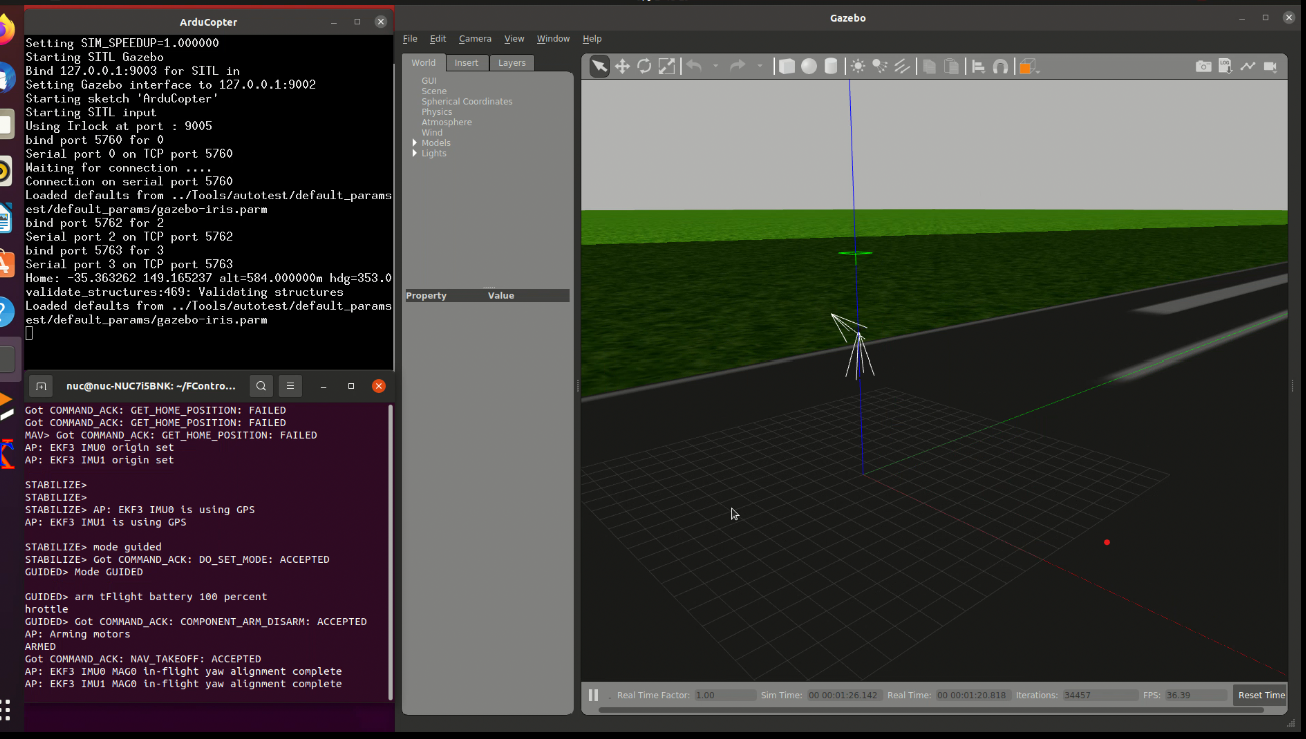
\includegraphics[width = 14cm]{fig/figure_chap7/apm1_simulation.png}
    \caption{基于Gazebo的单机仿真结果\label{fig:apm1_simulation}}
\end{figure}
单机联合仿真结果如\ref{fig:apm1_simulation}所示。

\subsection{基于Gazebo的双机仿真}
双机仿真主要用于验证两个无人机起飞同步性、航线飞行过程中的协调性、降落位置的精确度、两机位置过近时处理策略的可靠性。


\subsection{基于Gazebo的三机仿真}


\section{纵列式直升机试验平台设计及试验试飞}
协同吊挂系统中,单个飞行器的可控性和稳定性是整个系统安全性和可靠性的保障。因此,我们首先进行了纵列式直升机试验平台的设计和试验试飞工作。

\subsection{纵列式直升机试验平台设计}
电动双旋翼纵列式直升机总体参数见\ref{table:chap7:param}。

\begin{table}[htb!]
    \caption{小型纵列式直升机总体参数\label{table:chap7:param}}
    \begin{tabular}{cccc}
        \hline 指标 & 数值 & 指标 & 数值\\
        \hline 起飞重量(kg) & 18 & 空机重量(kg) & 8 \\
         电池重量(kg) & 6 & 载荷(kg) & 4 \\   
        \hline 电池电压(V) & 44.4 & 电池容量(KW*h) & 1.9\\
        \hline 旋翼直径(m) & 1.6 & 旋翼弦长(m) & 0.072\\
        扭转角(\degree) & -8 & 旋翼转速(rpm) & 1300\\
        桨叶片数 & 2 & & \\
        \hline 悬停时间(min) & 20 & & \\
        续航时间(min) & 30 & 最大速度(m/s) & 20 \\
        \hline
    \end{tabular}
\end{table}

见图\ref{fig:chap7:layout},无人直升机主要系统包含动力系统、传动系统、航电系统、能源系统、操纵系统、任务设备以及发射回收系统,这些系统均需布置在机身内部。系统内部布置需要布置和协调各主要系统的相对位置和尺寸,有利于结构的设计及控制较小的结构重量,实现气动布局和重心定位要求。除此之外,还需要满足可靠性、维护性以及工艺性等方面要求。

电动纵列双旋翼无人直升机内部布置纵向展开,全机可以分为前部机身、中部机身及尾部机身三部分。前机身主要布置了前旋翼升力系统、前旋翼操纵系统、任务设备与部分航电设备。中部机身是主承力结构件,承接了前后旋翼的气动力与全机的惯性力,在中部机身布置动力传动系统与能源系统。尾部机身布置有后旋翼升力系统、后旋翼操纵系统与部分航电设备,与前部机身类似。通过全机布置,无人直升机重心位于前后旋翼中间位置,满足设计要求。
\begin{figure}[htb!]
    \centering
    \subfloat[内部布置]{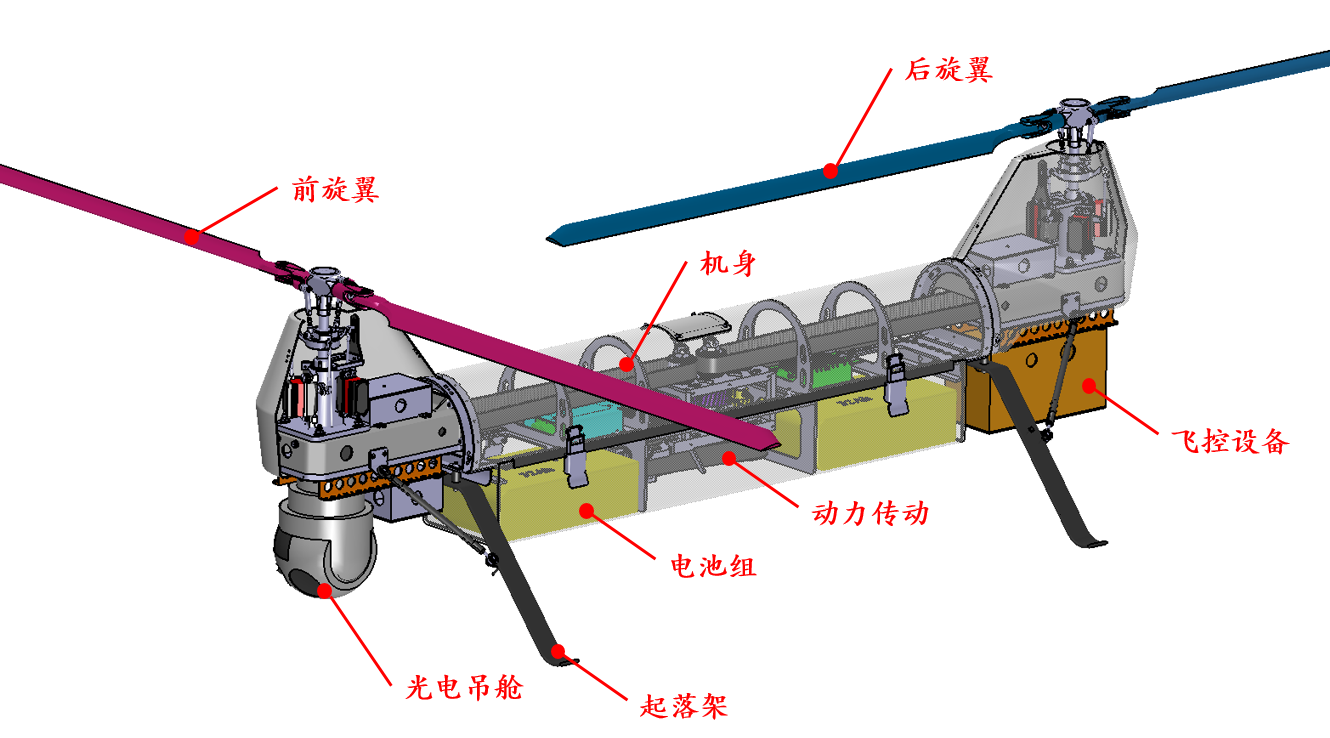
\includegraphics[width = 8cm]{fig/figure_chap7/structure.png}}\\
    \subfloat[前机身布置]{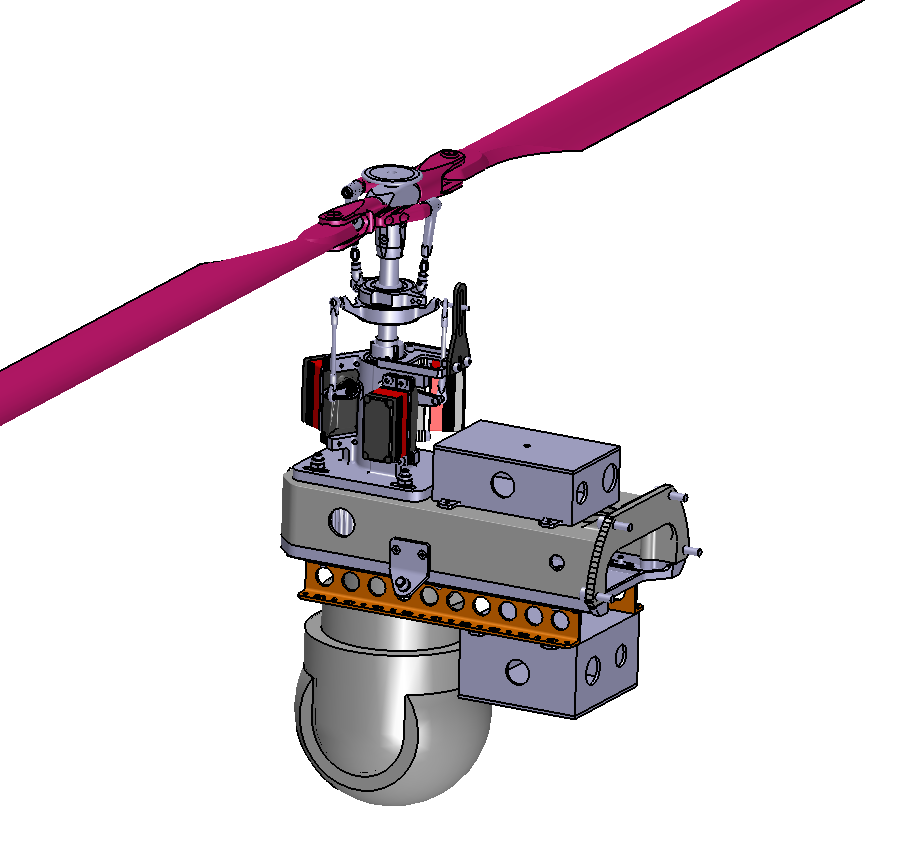
\includegraphics[width = 4cm]{fig/figure_chap7/front_fuse.png}}\quad
    \subfloat[中机身布置]{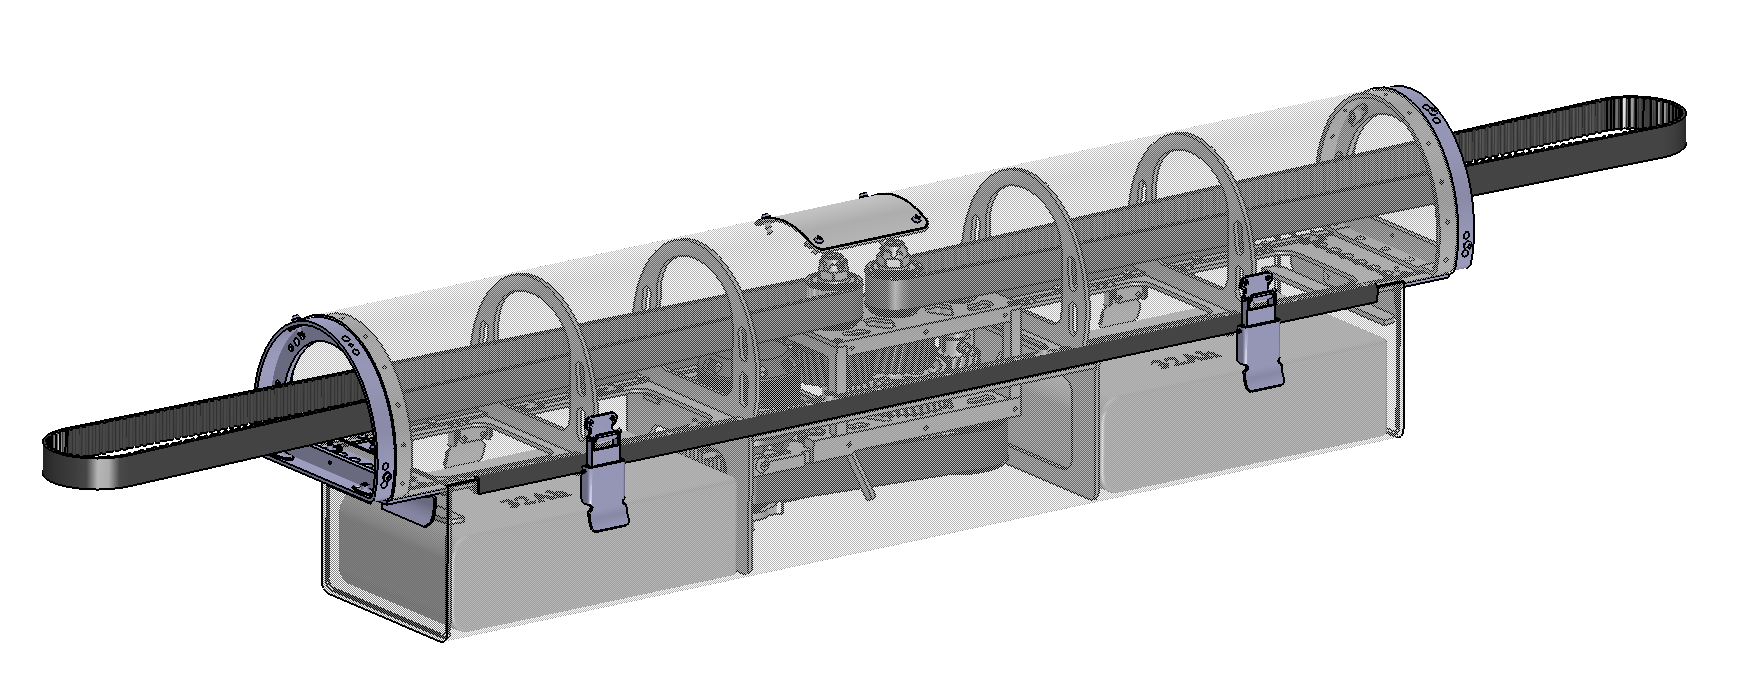
\includegraphics[width = 7cm]{fig/figure_chap7/mid_fuse.png}}
    \caption{纵列式无人直升机平台布置\label{fig:chap7:layout}}
\end{figure}

选用1台Kontronik PYRO 850-40L无刷电机作为无人直升机的动力。无刷电机结构紧凑、尺寸小、转动平稳,且使用维护简单。此无刷电机KV值为500 rpm/V,磁极数为14,最大转速为25000 rpm,内阻为0.016 $\Omega$。图\ref{fig:chap7:motor}给出了Kontronik 850-40L无刷电机的效率云图和特性图。其中,考虑到试验试飞过程中,纵列式直升机一般保持定转速变桨距的操纵方式,且油门通道一般在80\%左右,所以电机特性图是在电机输入电压为35.5 V(约为总电池电压的80\%)时绘制的。从图中可以看出,电机达到最大效率0.92时,电机转速为15306.44 rpm,电流为105.87 A,输出功率为3878.99 W。从表\ref{table:chap7:param}可知,期望旋翼转速为1300 rpm,所以减速比设置为11.8。

\begin{figure}[htb!]
    \centering
    \subfloat[电机效率云图]{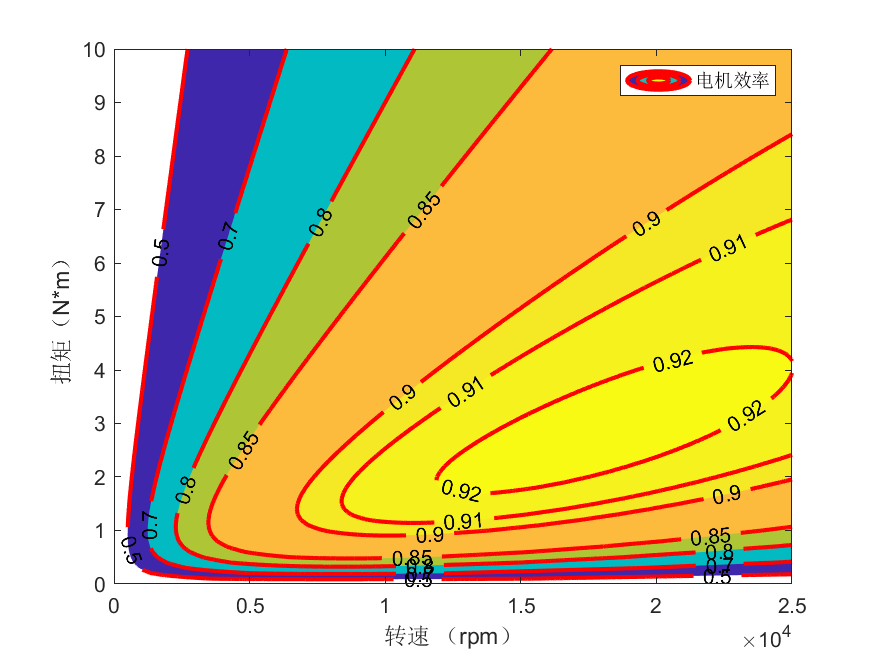
\includegraphics[width = 7cm]{fig/figure_chap7/motor1.png}}\quad
    \subfloat[电机特性图]{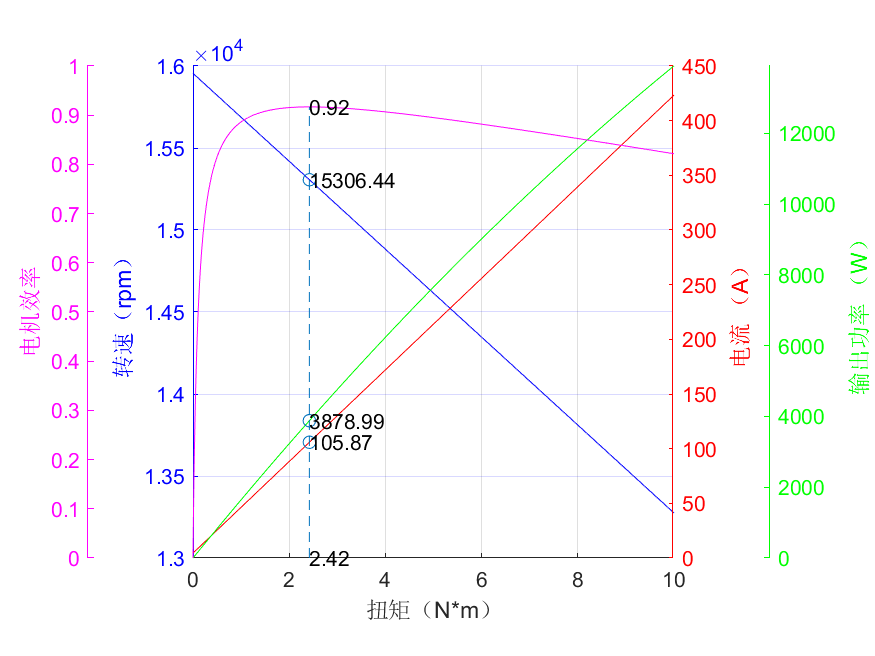
\includegraphics[width=7cm]{fig/figure_chap7/motor2.png}}
    \caption{电机效率云图和电机特性图\label{fig:chap7:motor}}
\end{figure}

为实现11.8的减速比及前后旋翼反向旋转,设计图\ref{fig:chap7:transfer}所示的传动方案。可见,全机包含3级减速,第一级为同步带减速,由电机动力经同步带传递至齿轮组,减速比为21:40;第二级为齿轮计算,减速比为20:44,同时完成旋转反向;第三极为同步带减速,减速比为24:67,将动力传递至前后双旋翼,实际旋翼转速为1308.4 rpm。
\begin{figure}[htb!]
    \centering
    \subfloat[]{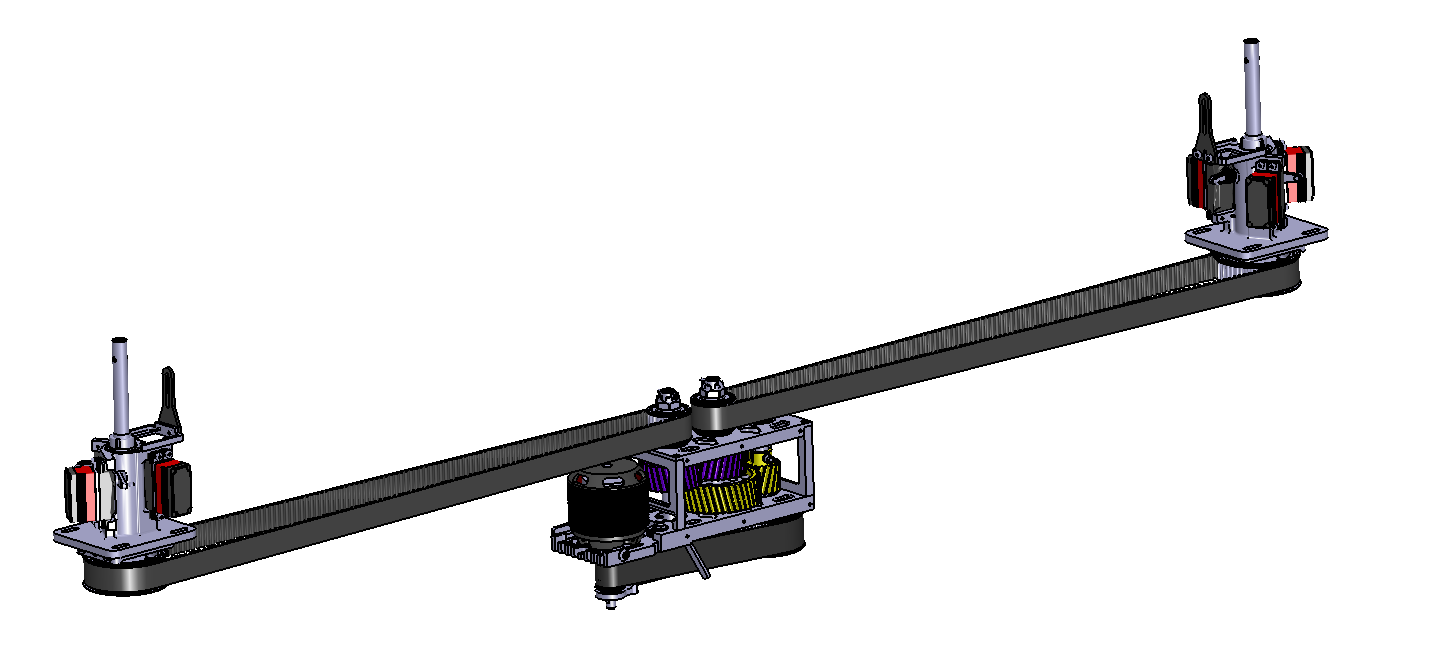
\includegraphics[width = 7cm]{fig/figure_chap7/transfer1.png}}\quad
    \subfloat[]{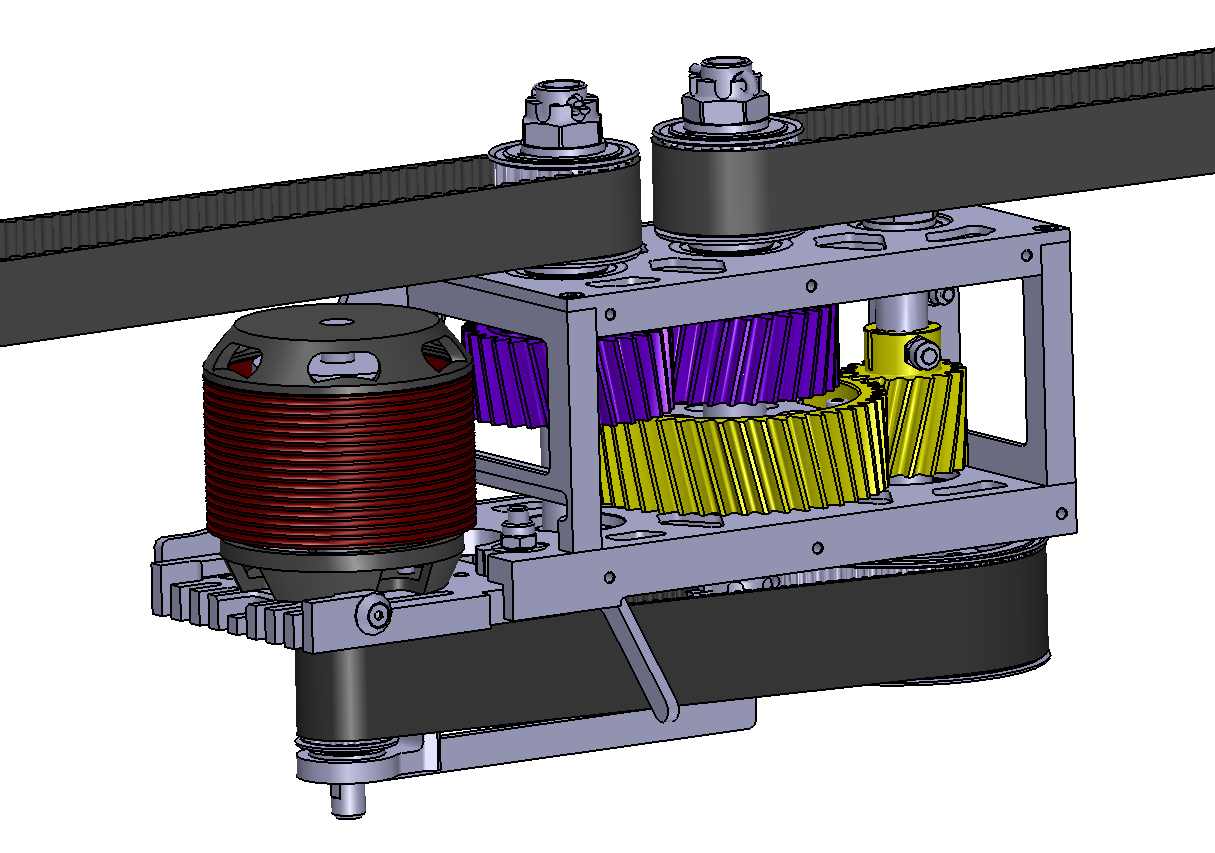
\includegraphics[width = 3cm]{fig/figure_chap7/transfer2.png}}\quad
    \subfloat[]{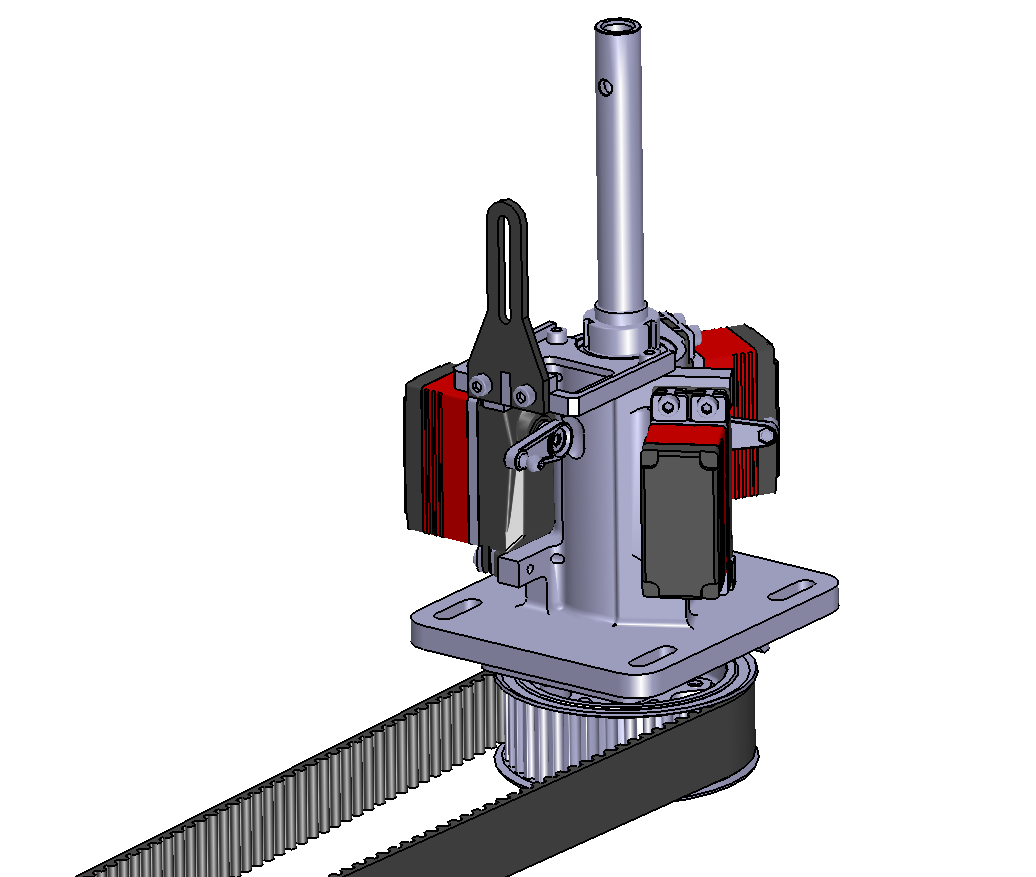
\includegraphics[width = 3cm]{fig/figure_chap7/transfer3.png}}
    \caption{小型纵列式直升机传动机构\label{fig:chap7:transfer}}
\end{figure}

纵列式直升机的垂向操纵通过同时加大或减小前后旋翼的总距来实现,纵向操纵通过前后旋翼总距差动实现,横向操纵通过同时加大或减小前后旋翼的横向周期变距实现,航向操纵通过前后旋翼横向周期变距差动来实现。前后旋翼头分别有3个舵机,采用H-3布置方式,即舵机间相隔120 \degree。

图\ref{fig:chap7:elec}是无人机上航电系统的线路连接示意图。从图中可以看出所有的电源负极都是共地的,用来消除电势差所造成的影响。而且在各个传感器附近,尽量不要有大的电流通过,以防止大电流产生磁场,对传感器造成影响,使得飞控取得传感器的数据有较大的偏差。共有6个舵机,对应上文提到的前后旋翼头上的舵机,油门信号直接输出到电机电调,进而通过传动系统驱动旋翼旋转。
\begin{figure}[htb!]
    \centering
    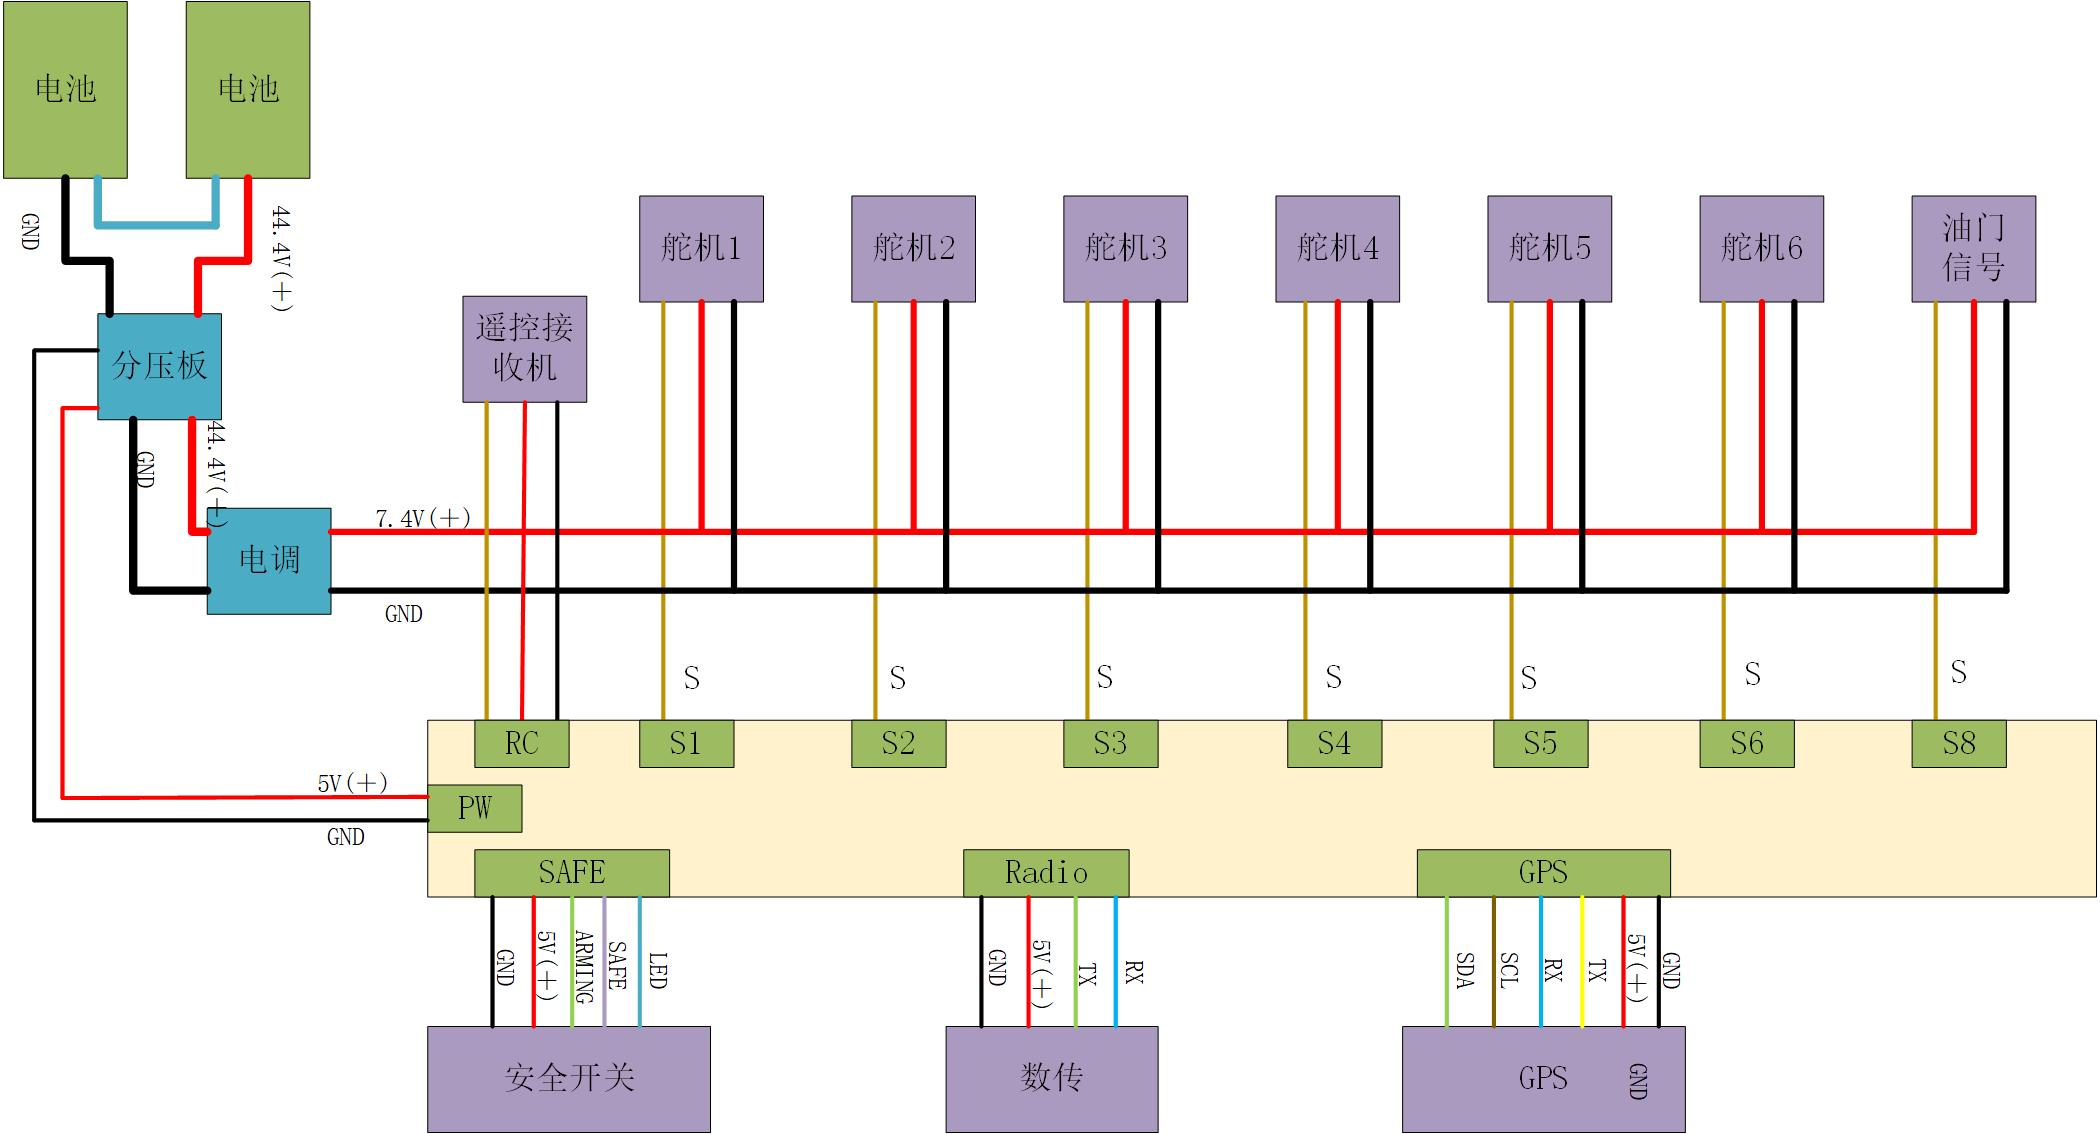
\includegraphics[width = 10cm]{fig/figure_chap7/electric.jpg}
    \caption{航电系统连接方式\label{fig:chap7:elec}}
\end{figure}

根据设计图纸完成电动纵列双旋翼无人直升机的制造与装配工作,布置航电系统,并开展相关的试飞试验,见图\ref{fig:chap7:tandem}。
\begin{figure}[htb!]
    \centering
    \subfloat[]{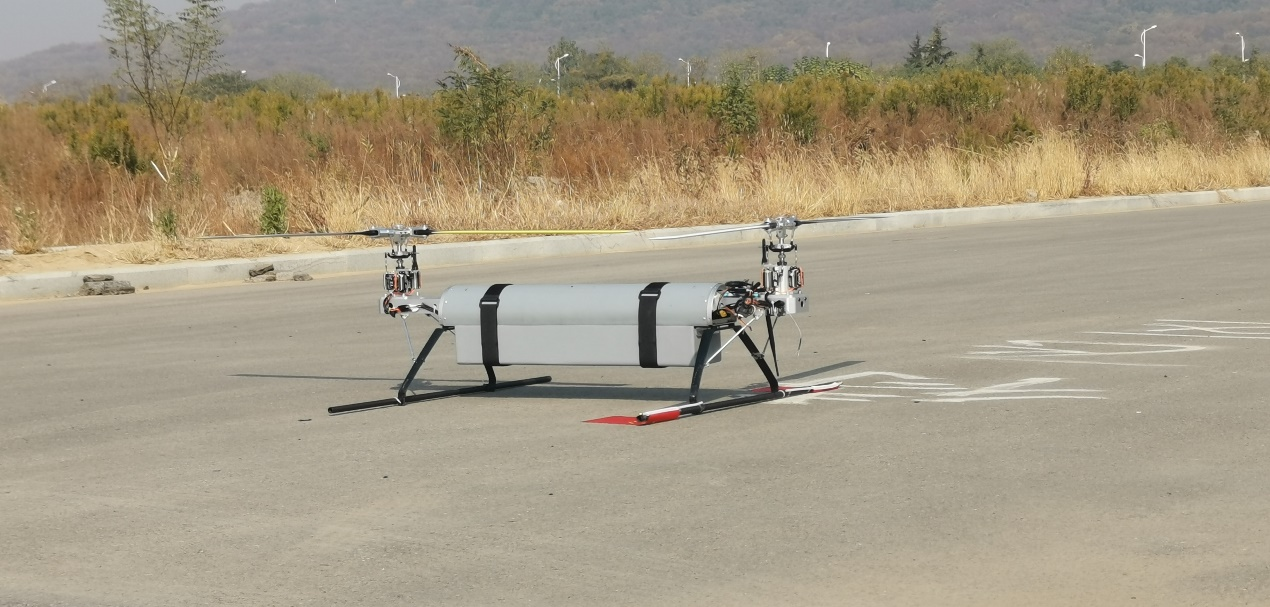
\includegraphics[width = 7cm]{fig/figure_chap7/tandem1.jpg}}\quad
    \subfloat[]{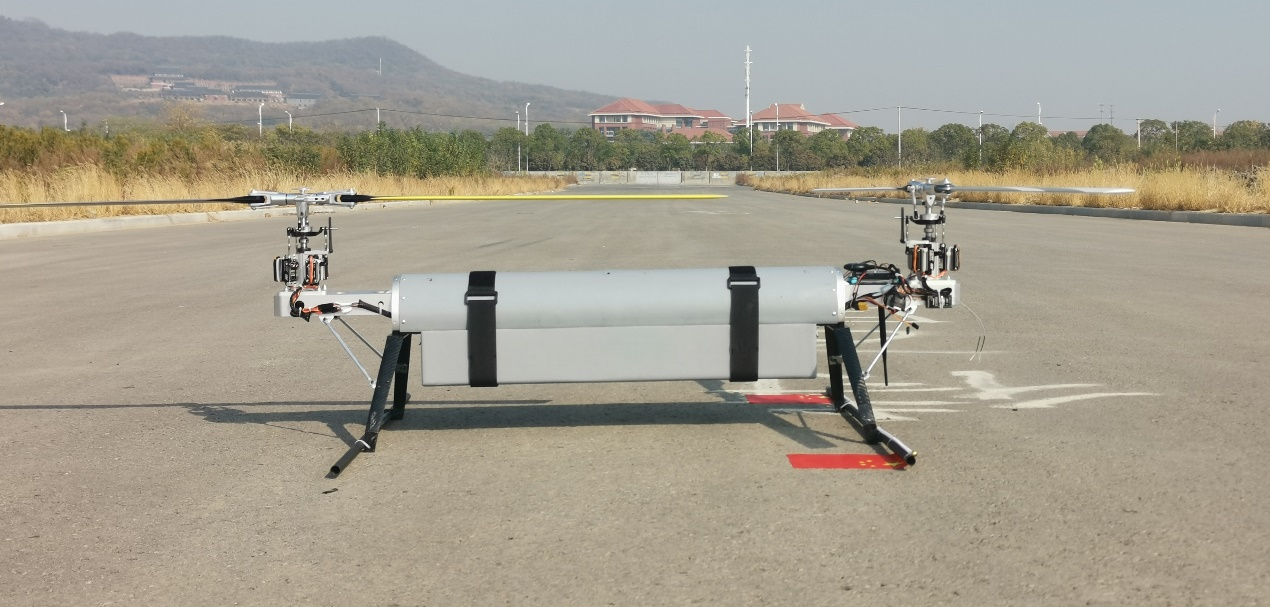
\includegraphics[width = 7cm]{fig/figure_chap7/tandem2.jpg}}\\
    \subfloat[]{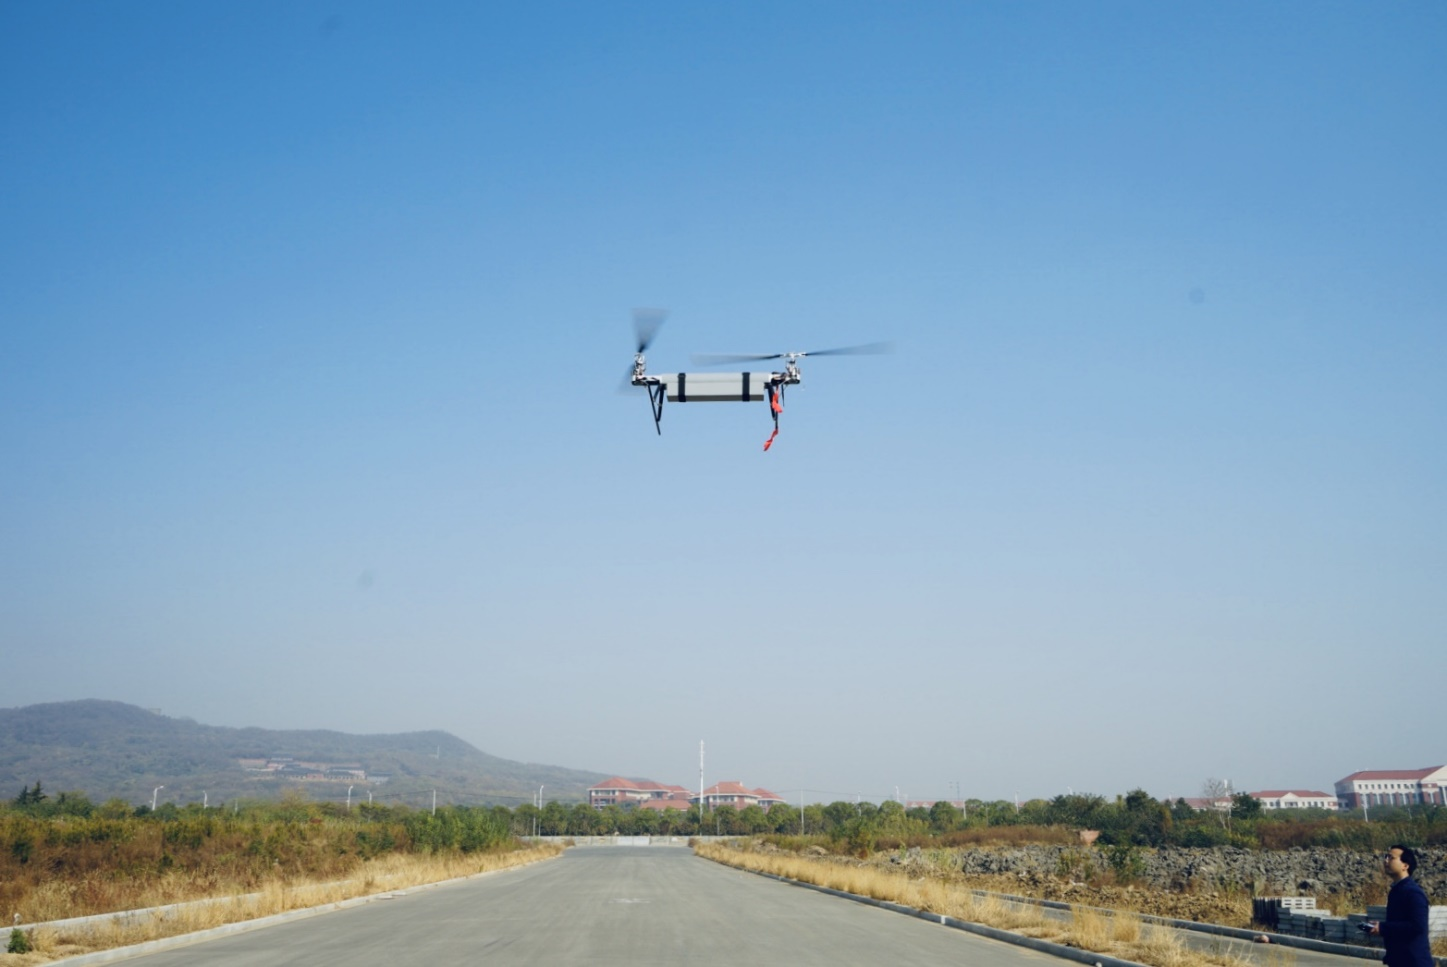
\includegraphics[width = 7cm]{fig/figure_chap7/tandem3.jpg}}\quad
    \subfloat[]{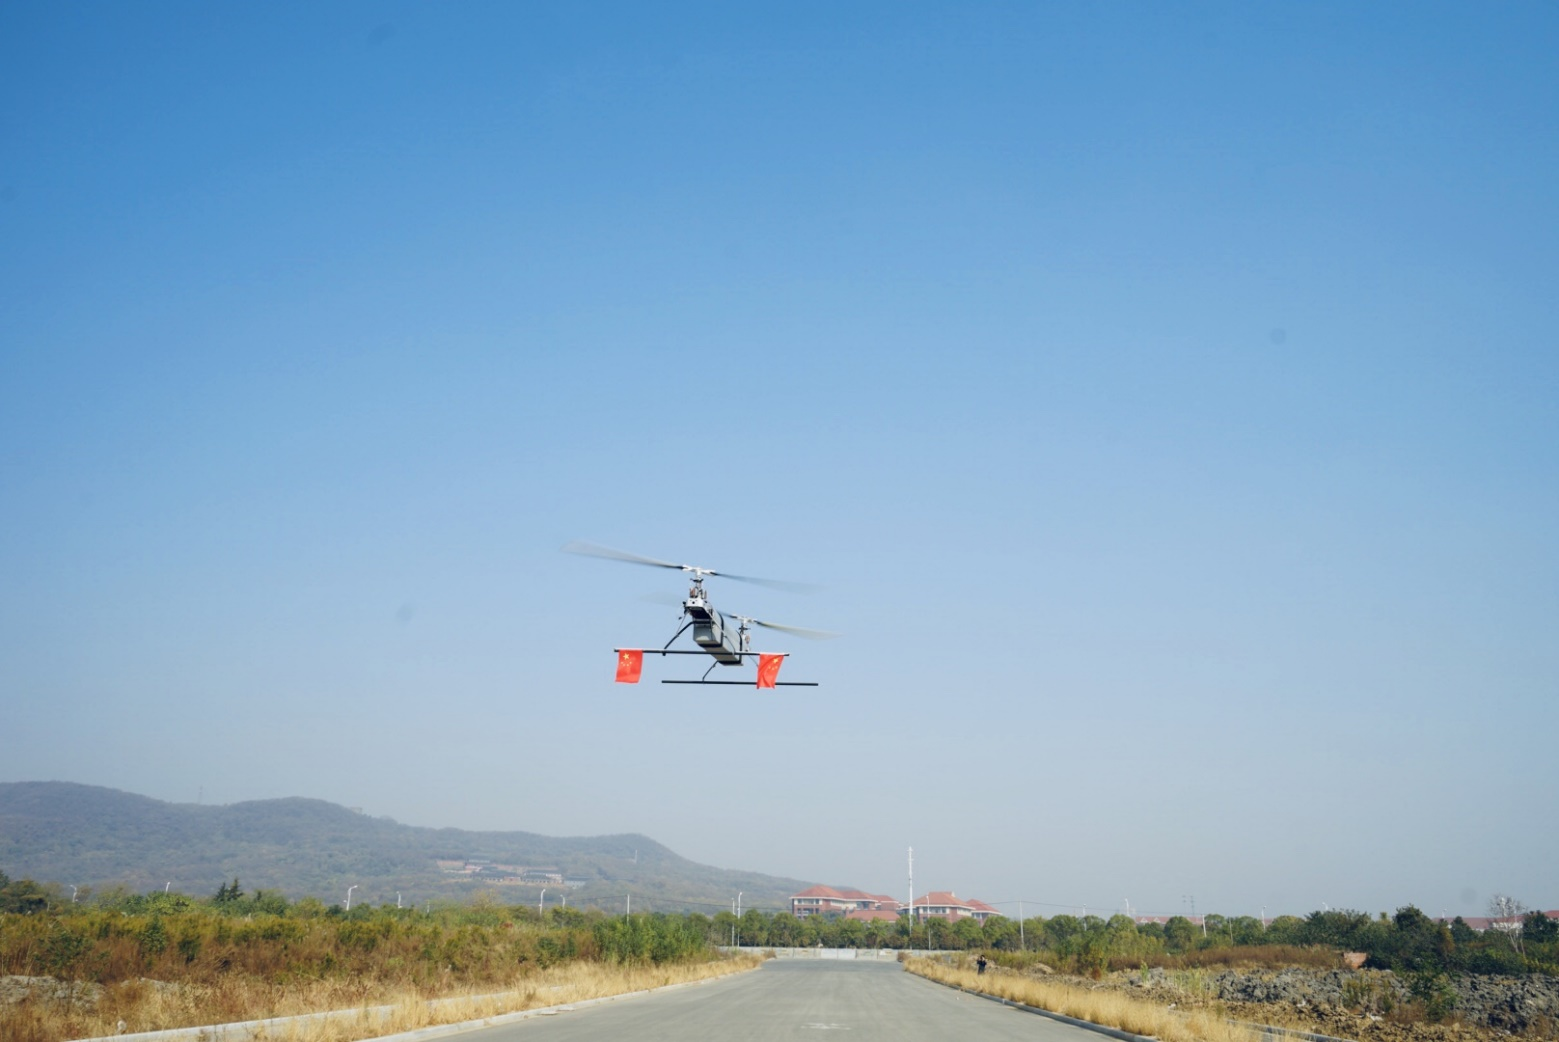
\includegraphics[width = 7cm]{fig/figure_chap7/tandem4.jpg}}
    \caption{小型纵列式直升机试验试飞图\label{fig:chap7:tandem}}
\end{figure}

\subsection{纵列式直升机姿态增稳控制验证}
图\ref{fig:chap7:ATT}给出姿态增稳飞行时小型纵列式直升机的姿态跟随情况,从图中可以看出技术验证机的姿态能够很好的跟随遥控器的输入,并且飞行器在飞行的过程中能够很好的保持姿态的平稳,姿态角的变化量都保持在一个很小的角度内。此外,偏航角存在跳变,是偏航角达到360 \degree 会变为0 \degree 所致。
\begin{figure}[htb!]
    \centering
    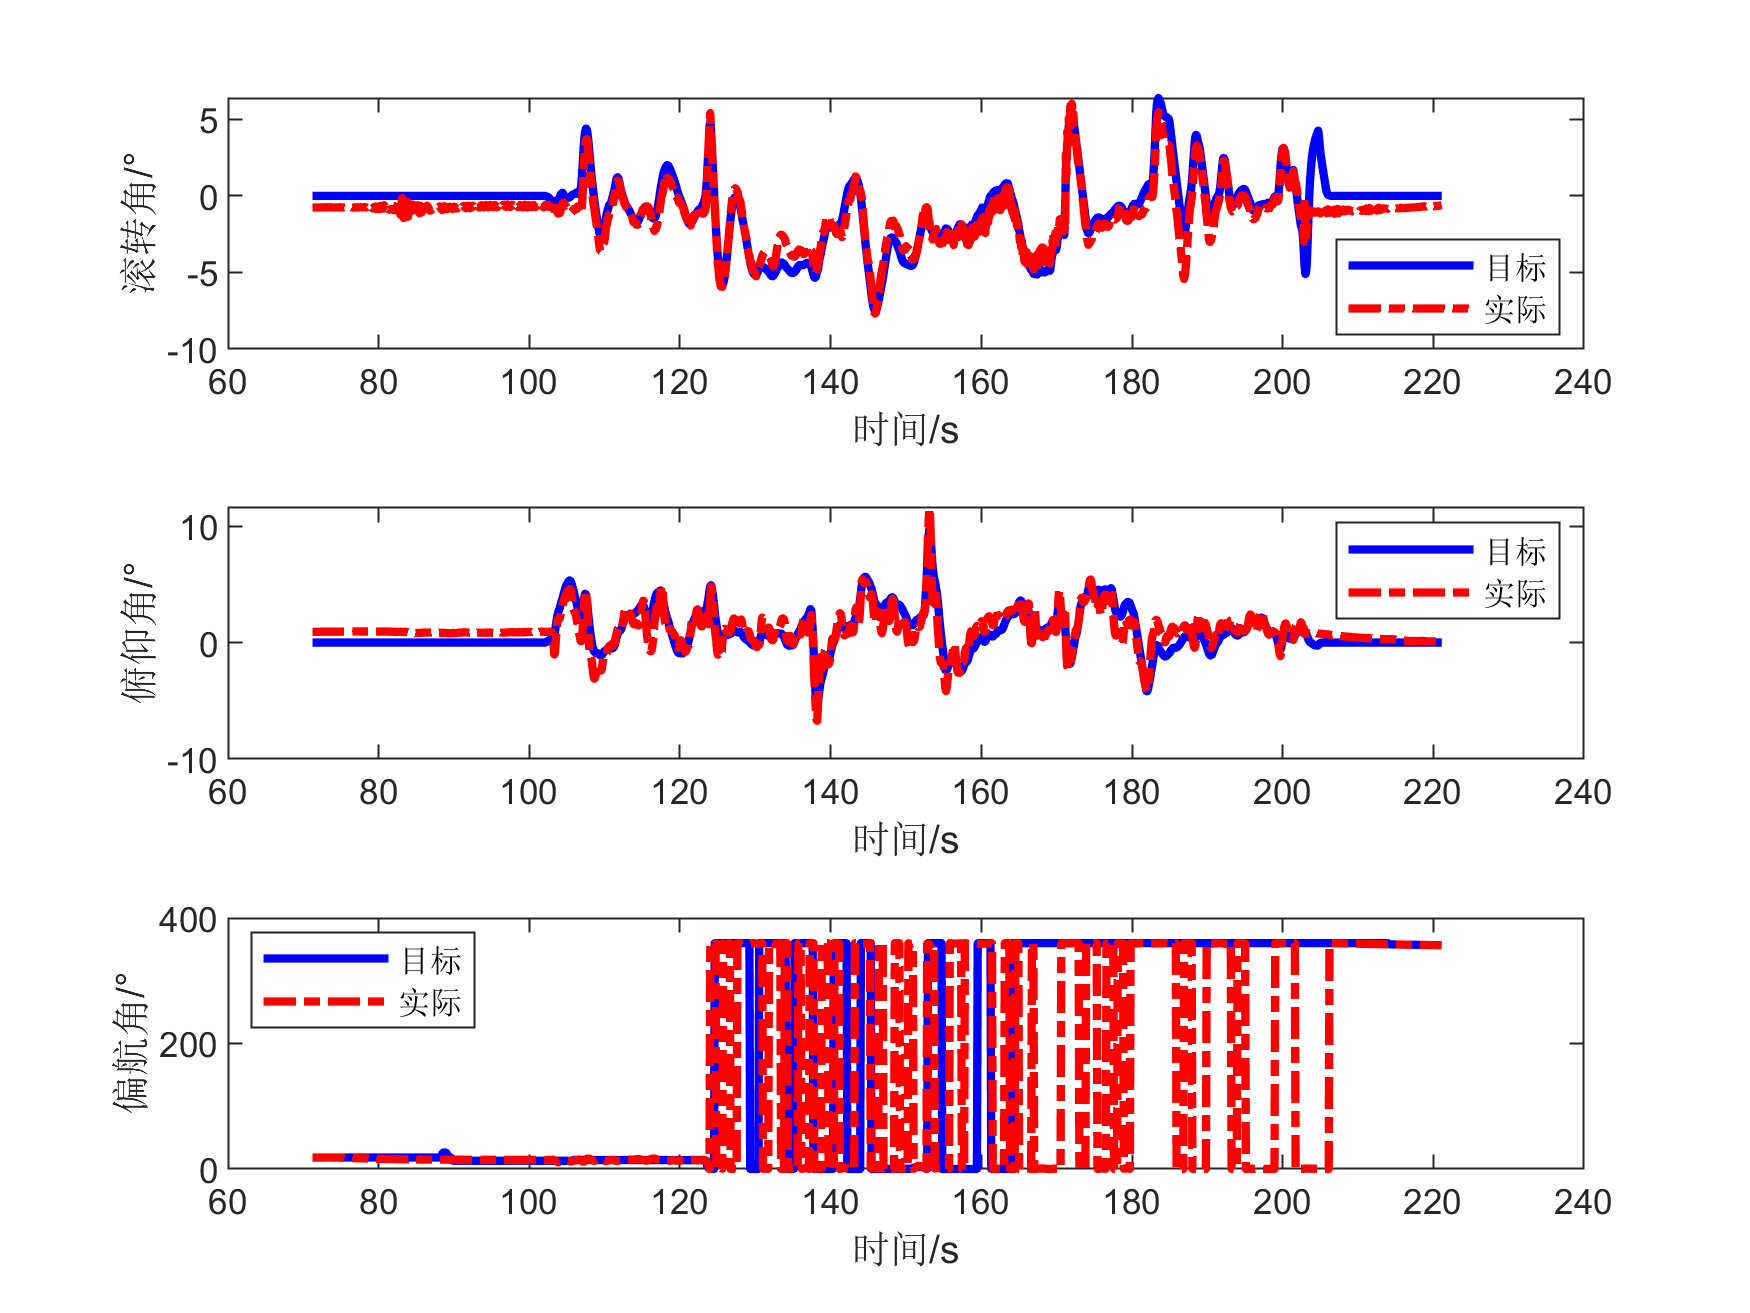
\includegraphics[width = 14cm]{fig/figure_chap7/ATT.png}
    \caption{纵列式直升机姿态跟随情况\label{fig:chap7:ATT}}
\end{figure}

可见,设计的纵列式直升机具备良好的姿态跟随能力,可以进一步进行悬停、自主航线、协同吊挂飞行的试验试飞。
\subsection{纵列式直升机悬停、航线飞行能力验证}
图\ref{fig:chap7:hover}为纵列式直升机自主悬停时前向位置、横向位置、高度的变化情况。图中位置变化通过将GPS测量的经纬度信息转换得到。从图中可以看出,相对于原点位置,前向、横向的位移变化不超过0.5m;高度保持在10m,最大位移变化不超过0.5m,满足自主悬停试飞要求。
\begin{figure}[htb!]
    \centering
    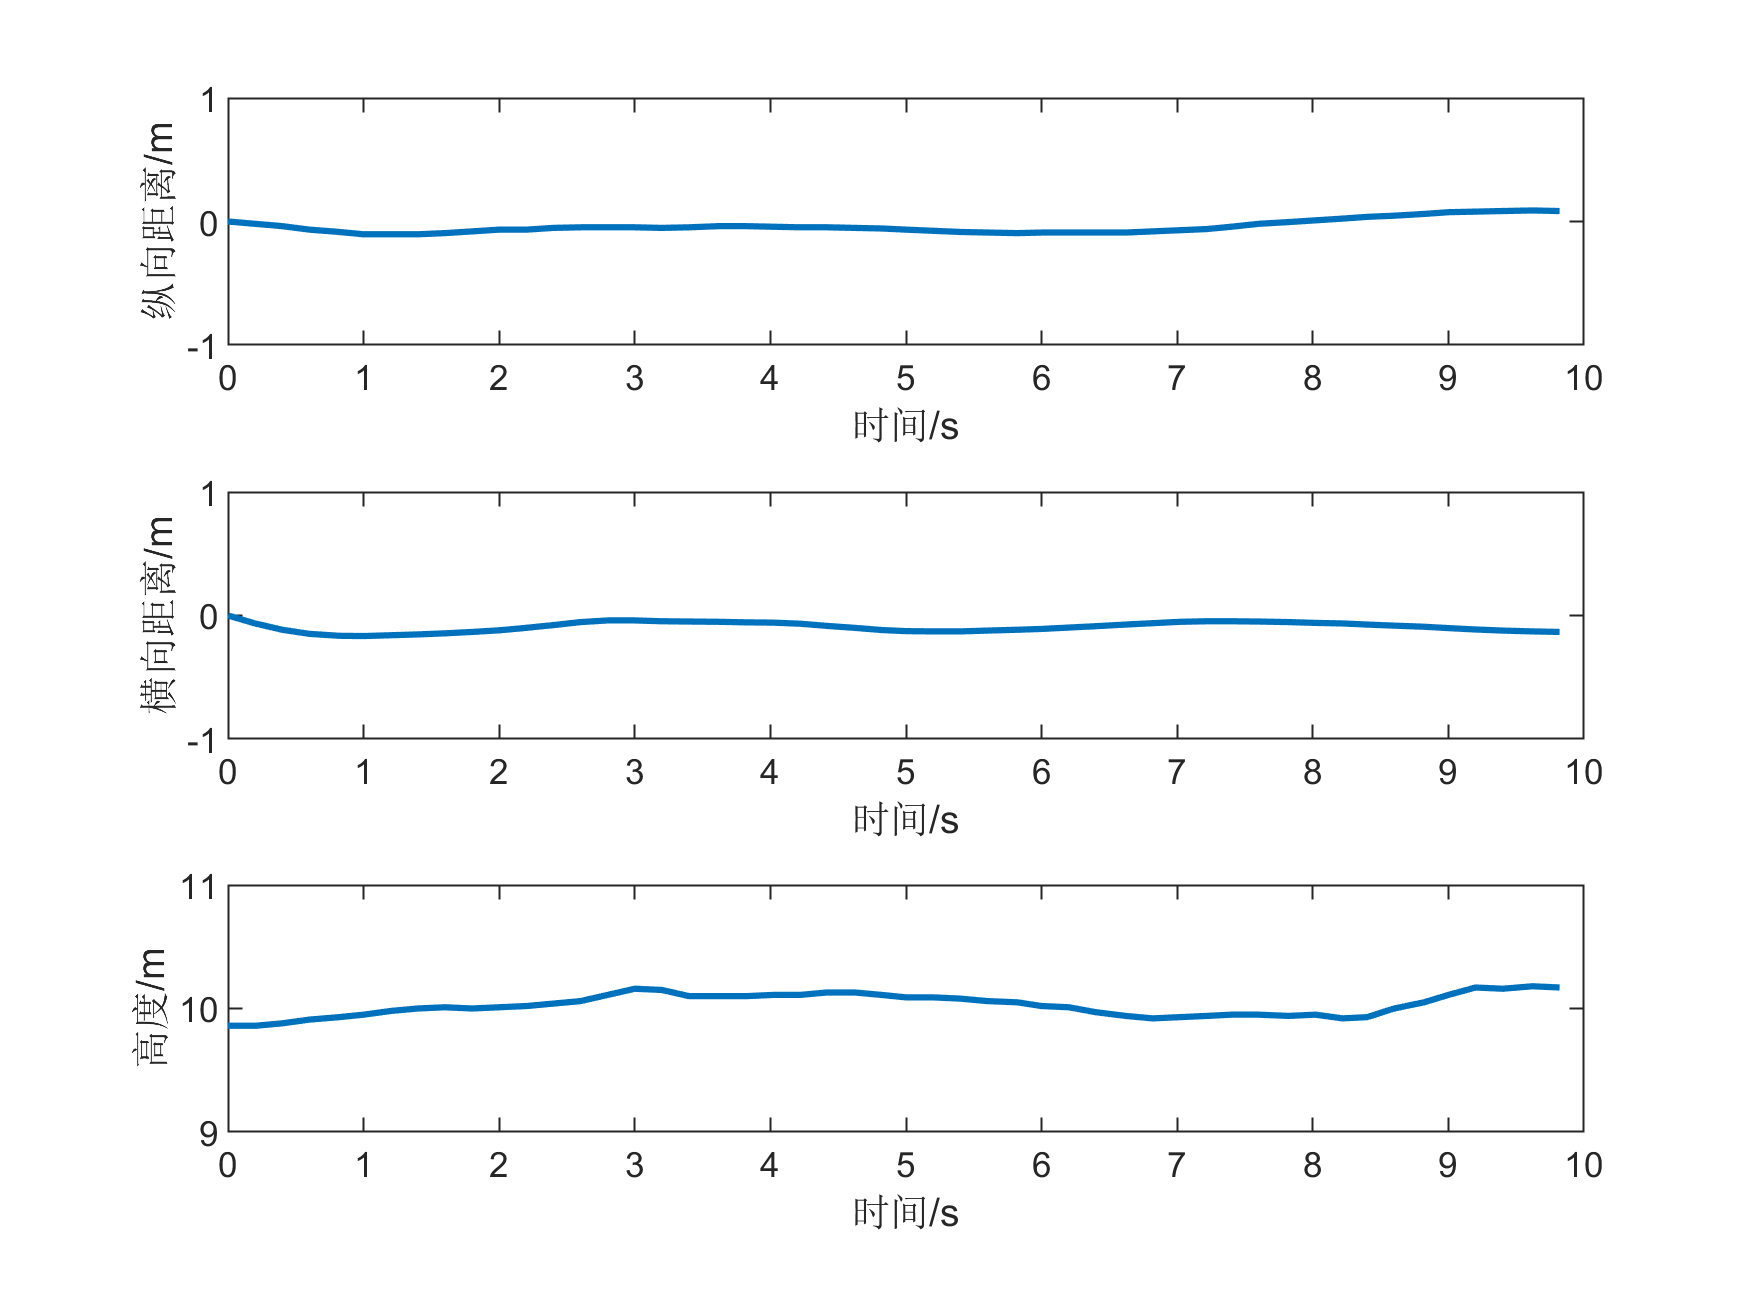
\includegraphics[width = 14cm]{fig/figure_chap7/hover.png}
    \caption{纵列式直升机自主悬停时的位置变化\label{fig:chap7:hover}}
\end{figure}

前飞后退任务为:纵列式直升机前飞100m后悬停,期间保持姿态平稳,最大速度大于30公里/小时(8.33m/s);接着后退100m,依旧保持姿态平稳。

图\ref{fig:chap7:cruise}给出了纵列式直升机,前飞距离、高度、前飞速度随时间的变化情况。从图中可以看出,22s至45s左右纵列式直升机完成前飞运动,随后保持悬停10s,55s到78s左右完成后退。期间,纵列式直升机保持在10m高度,最大偏移不超过1m。飞行速度(绝对值)22s到45s先增加后减小,55s到78s先减小后增加。整个飞行过程中,最大飞行速度为9.2m/s左右。
\begin{figure}[htb!]
    \centering
    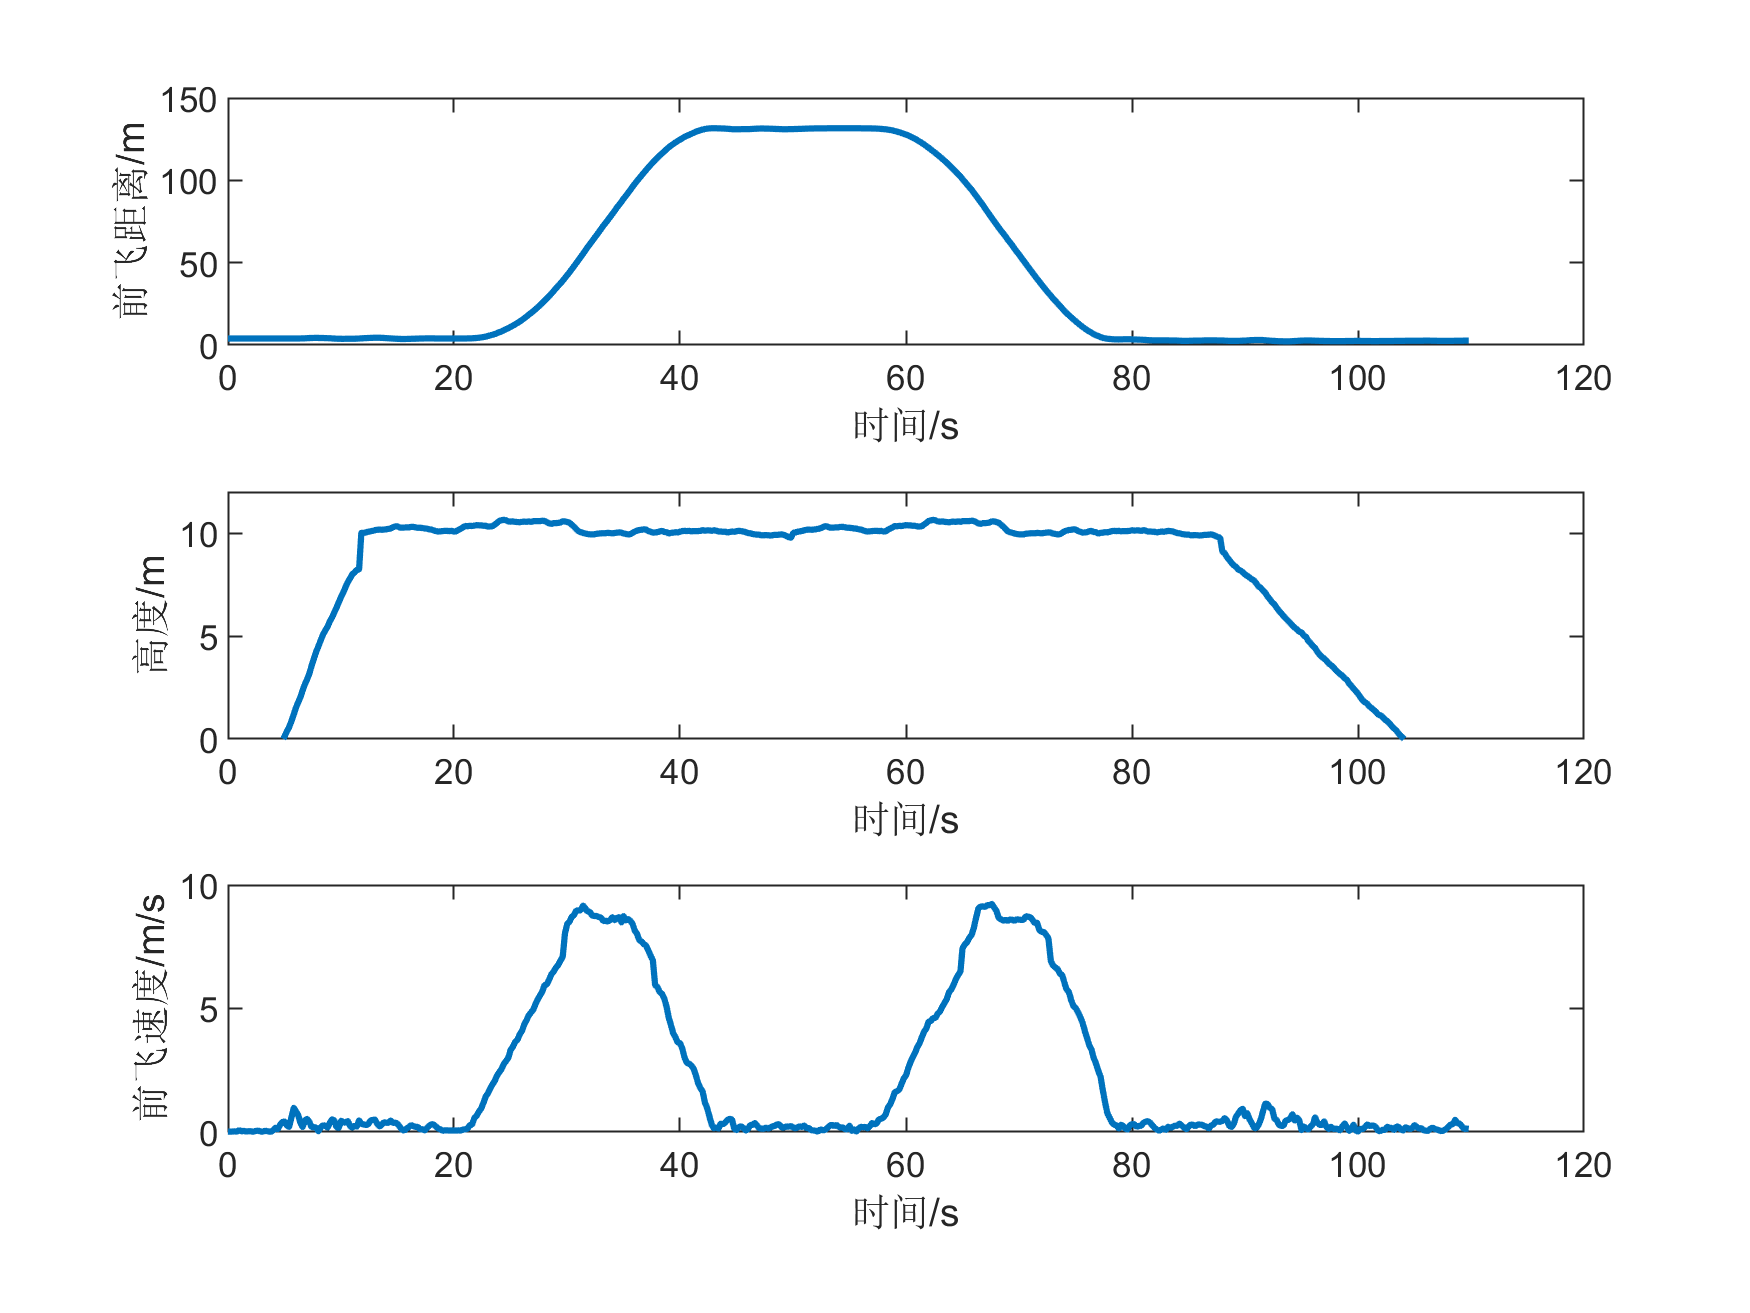
\includegraphics[width = 14cm]{fig/figure_chap7/cruise.png}
    \caption{纵列式直升机前飞后退时的位置和速度变化\label{fig:chap7:cruise}}
\end{figure}

可见,设计的纵列式直升机具备定点飞行、悬停、航线飞行的能力,为接下来的试验试飞奠定了基础。

\subsection{纵列式直升机吊挂能力验证}
\section{单旋翼带尾桨直升机试验试飞}
\subsection{单旋翼带尾桨直升机增稳控制验证}
\subsection{单旋翼带尾桨直升机航线飞行能力验证}
\section{双四轴无人机带吊挂试验试飞}
为验证以吊挂物为中心的分层协同吊挂控制策略的可靠性,考虑试验成本,首先开展了双四轴无人机带吊挂试验试飞工作。
\section{直升机协同吊挂试验试飞}
\section{本章小结}
                                                                                       